\documentclass{article}
\usepackage[dvipsnames,svgnames]{xcolor}
\usepackage[colorlinks=true,linkcolor=Blue,urlcolor=Blue,citecolor=Blue,anchorcolor=Blue]{hyperref}
\usepackage{arxiv}

%% Language and font encodings
\usepackage[utf8]{inputenc} % allow utf-8 input
\usepackage[T1]{fontenc}    % use 8-bit T1 fonts
\usepackage{hyperref}       % hyperlinks
\usepackage{url}            % simple URL typesetting
\usepackage{booktabs}       % professional-quality tables
\usepackage{amsfonts}       % blackboard math symbols
\usepackage{nicefrac}       % compact symbols for 1/2, etc.
\usepackage{microtype}      % microtypography
\usepackage{lipsum}         % Can be removed after putting your text content
\usepackage{float}
\usepackage[style=authoryear,backend=biber]{biblatex}
\bibliography{references}

\usepackage{graphicx}
% \usepackage{doi}


\begin{document}

\begin{titlepage}
\centering
{\LARGE\bfseries LLM-Augmented Knowledge-Graph-Based Recommendation System}

\vspace{1.5cm}

{\Large By}

{\Large Kartikey Chauhan

501259284 }

\vspace{2cm}
{\Large Literature Review \& 


Exploratory Data Analysis 
}

\vspace{2cm}

{\Large Master of Science

in the Program of 

Data Science and Analytics

}

\vspace{2cm}
{\Large Toronto, Ontario, Canada, 2024}

\vfill

{\itshape © Kartikey Chauhan, 2024}
\end{titlepage}

\pagenumbering{roman}
\setcounter{page}{2}

\tableofcontents
\listoffigures
\listoftables


\fancyhf{}
\renewcommand{\headrulewidth}{0pt}
\fancyfoot[R]{\thepage}
\renewcommand{\footrulewidth}{0pt}
\pagenumbering{arabic}

\section{Introduction}

This document covers the Introduction, Literature Review and Exploratory Data Analysis for the first deliverable of Major Research Project (MRP). It begins with a brief background on the topic and datasets, defines the problem, and states the research question. This is followed by a literature review and a detailed exploratory analysis of the dataset.

\subsection{Background}
Recommender systems have been widely applied to address the issue of information overload in various internet services, exhibiting promising performance in scenarios such as e-commerce platforms and media recommendations. 
In the general domain, the traditional knowledge recommendation method is \textit{collaborative filtering (CF)}, which usually suffers from the cold start problem and sparsity of user-item interactions. 
Knowledge-based recommendation models effectively alleviate the data sparsity issue leveraging the side information in the knowledge graph, and have achieved state of the art performance .
However, KGs are difficult to construct and evolve by nature, and existing methods often lack considering textual information. On the other hand, LLMs are black-box models, which often fall short of capturing and accessing factual knowledge.
Therefore, it is complementary to unify LLMs and KGs together and simultaneously leverage their advantages.
This project aims to explore LLM-augmented KGs, that leverage Large Language models (LLM) for different KG tasks such as embedding, completion, construction and also incorporate textual information which could be a way to help overcome these challenges and lead to better recommendation systems.

\subsection{Research Objectives}
The research objectives of this project are to investigate the use of Large Language Models (LLMs) to enhance the construction, quality, and volume of information in knowledge graphs (KGs). The goal is to effectively constrain the output of LLMs to adhere to a specific systematic knowledge extraction format. Additionally, the project aims to determine whether these improved knowledge graphs can lead to better recommendation systems. Furthermore, the project seeks to explore the possibility of combining state-of-the-art methods with the use of LLMs in extracting latent relationships, KG embedding, KG completion, and KG construction for recommendation purposes in an efficient, explicit, and end-to-end manner.

\section{Literature Review}

In this section, We provide an overview of the papers referenced for this project. Knowledge Graphs (KGs) as a form of structured knowledge have drawn significant attention from academia and the industry (\cite{ji2022survey}). There have been several efforts to construct KGs to facilitate the discovery of relevant information within specific fields. Most of these efforts have focused on extracting information from text.

Our problem statement can be broken down into 3 main components: KG Construction, KG Embedding and Knowledge Graph-based Recommendation Systems. We will review the literature in these areas to understand the current state of the art and identify gaps that can be addressed in our research.

\subsubsection{Knowledge Graph-based Recommendation Systems}

In recommendation, KGs have been used to enhance the performance of recommendation systems by incorporating high-order connectivities from KGs into user-item interactions. \textbf{\cite{wang2019kgat}} introduce the \textbf{Knowledge Graph Attention Network (KGAT)}, which enhances recommendation systems by leveraging an attention mechanism to discern the significance of various neighbor connections, demonstrating superior performance and interpretability compared to existing models such as Neural FM and RippleNet through extensive experiments on multiple public benchmarks. The model's end-to-end approach efficiently captures and utilizes high-order relations, providing more accurate, diverse, and explainable recommendations.

\textbf{\cite{he2020lightgcn}} propose \textbf{LightGCN}, a lightweight graph convolutional network that simplifies the design of graph neural networks for collaborative filtering. LightGCN eliminates the feature transformation and nonlinear activation functions in traditional GCNs, focusing solely on the graph structure. The model achieves state-of-the-art performance on several recommendation benchmarks, outperforming more complex models such as NGCF and GAT. LightGCN's simplicity and efficiency make it an attractive choice for large-scale recommendation systems, demonstrating the effectiveness of collaborative filtering with graph neural networks.

\textbf{KUCNet} (\textbf{\cite{liu2024knowledgeenhanced}}) is a novel knowledge-enhanced recommendation method that constructs user-centric subgraphs from the collaborative knowledge graph to capture relevant information for each user. It uses graph neural networks to propagate representations on these subgraphs, learning user preferences from collaborative filtering signals and knowledge graph semantics. KUCNet outperforms existing collaborative filtering, knowledge graph-based, and collaborative knowledge graph-based recommendation methods, especially for the inductive setting with new users/items.


\subsubsection{Knowledge Graph Embedding}

\textbf{\cite{guo2020survey}} present a comprehensive survey of knowledge graph embedding techniques, which have been widely applied in various tasks such as recommendation, search, and question answering. The survey categorizes embedding methods into three groups: translation-based, semantic matching-based, and neural network-based. The authors provide a detailed overview of each category, discussing their strengths, weaknesses, and applications. The survey also highlights the challenges and future directions in knowledge graph embedding research, emphasizing the importance of incorporating textual information to enhance the quality and interpretability of embeddings.

\textbf{\cite{zhang2021kget}} introduce the \textbf{Knowledge Graph Embedding Transformer (KGET)}, a novel model that leverages the transformer architecture to learn embeddings for knowledge graphs. KGET incorporates a self-attention mechanism to capture complex relational patterns and dependencies in the graph structure. The model outperforms existing embedding methods such as TransE, DistMult, and ComplEx on several knowledge graph completion tasks, demonstrating its effectiveness in capturing long-range dependencies and semantic relationships. KGET's ability to model complex interactions between entities and relations makes it a promising approach for knowledge graph embedding.

\subsubsection{Knowledge Graph Construction}

\textbf{\cite{ji2022survey}} provide a comprehensive survey of knowledge graph construction methods, which aim to extract structured knowledge from unstructured text data. The survey categorizes construction methods into three groups: \textbf{rule-based}, \textbf{statistical}, and \textbf{neural network-based}. The authors discuss the strengths and weaknesses of each category, highlighting the challenges and future directions in knowledge graph construction research. The survey emphasizes the importance of incorporating textual information to enhance the quality and completeness of knowledge graphs, providing valuable insights for researchers and practitioners in the field.

\subsubsection{Knowledge Graph Construction with Large Language Models}
However, the traditional KG construction methods often lack the ability to incorporate textual information, which is essential for capturing the rich semantics and context of entities and relations. 

Several studies have explored the integration of of current language models like \textbf{BERT} with knowledge graphs to enhance the quality and efficiency of knowledge representation and recommendation systems.

\textbf{\cite{xu2021text2kg}} propose a novel method for constructing knowledge graphs from text, called \textbf{Text2KG}. Text2KG utilizes a pre-trained language model to extract structured knowledge from unstructured text data, generating entity and relation triples for constructing knowledge graphs. The model achieves competitive performance on knowledge graph construction tasks, outperforming existing methods such as OpenIE and ReVerb. Text2KG's ability to extract high-quality knowledge from text data demonstrates its potential for automating the construction of knowledge graphs from large-scale text corpora.

\textbf{\cite{zhang2021kgbert}} introduce \textbf{KG-BERT}, a pre-trained language model that incorporates knowledge graph embeddings to enhance the representation learning of entities and relations. KG-BERT leverages the pre-trained BERT model to capture contextual information from text data and knowledge graph embeddings to capture structured information from knowledge graphs. The model achieves state-of-the-art performance on several knowledge graph completion tasks, demonstrating its effectiveness in capturing both textual and structured information. KG-BERT's ability to leverage both text and knowledge graph embeddings makes it a promising approach for enhancing the quality and interpretability of knowledge graph embeddings.

The emergence of Large Language Models (LLMs) has revolutionized research and practical applications by enabling complex reasoning and task generalization through techniques like In-Context Learning and Chain-of-Thought. LLMs offer promising solutions to existing recommender system challenges, such as poor interactivity, explainability, and the cold start problem, by generating more natural and cross-domain recommendations and enhancing user experience through stronger feedback mechanisms.

As such, the integration of LLMs with KGs presents a novel direction to overcome the limitations of traditional KGs, such as the challenge of incorporating textual information. 

\textbf{\cite{ullah2021llm-kgc}} introduce a novel method for knowledge graph completion using large language models, called \textbf{LLM-KGC}. LLM-KGC leverages the pre-trained language model BERT to predict missing relations in knowledge graphs, capturing complex relational patterns and dependencies. The model outperforms existing knowledge graph completion methods such as TransE, DistMult, and ComplEx on several benchmark datasets, demonstrating its effectiveness in capturing long-range dependencies and semantic relationships. LLM-KGC's ability to leverage large language models for knowledge graph completion makes it a promising approach for enhancing the quality and completeness of knowledge graphs.

\textbf{\cite{pan2023unifying}} discuss different approaches to unify large language models (LLMs) and knowledge graphs (KGs) to leverage their complementary strengths. Several methods are covered:

% \begin{figure}[H]
%   \centering
%   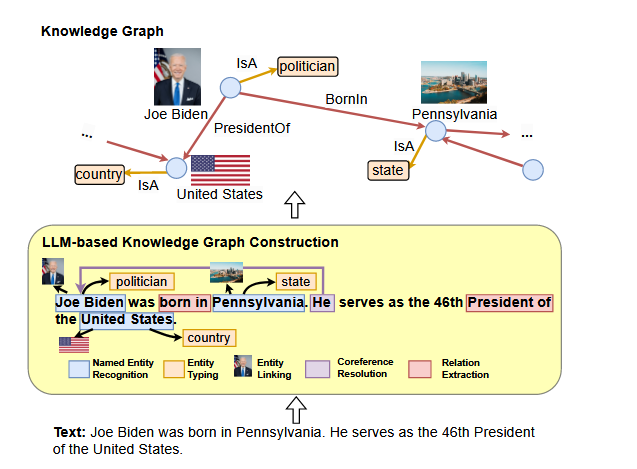
\includegraphics[width=0.8\textwidth]{img/KG_construction.png}
%   \caption{The general framework of LLM-based KG construction. From \cite{pan2023unifying}.}
%   \label{fig:kg_construction}
%   \end{figure}


\textbf{Integrating KGs into LLM Training}
\begin{itemize}
  \item Injecting KG information into LLM pre-training objectives, e.g. entity/relation prediction tasks. 
  \item Concatenating linearized KG triples with text as input to LLMs. 
\end{itemize}

\textbf{Using LLMs for Knowledge Graph Embeddings}
\begin{itemize}
  \item Using LLMs to encode textual descriptions of entities/relations into embeddings for knowledge graph embedding methods. 
  \item Masked language modeling approaches to encode KG triples. 
\end{itemize}

\textbf{Using LLMs for Knowledge Graph Completion}
\begin{itemize}
  \item Encoder-decoder or decoder-only LLMs that generate the missing entity in a triple. 
\end{itemize}

\textbf{Using LLMs for KG-to-Text Generation}
\begin{itemize}
  \item Fine-tuning LLMs like BART and T5 on linearized KG inputs to generate text descriptions. 
  \item Injecting structure-aware KG representations into seq2seq LLMs. 
\end{itemize}


\subsubsection{Other LLM-Augmented Recommendation Systems}
Apart from KG construction and embedding, LLMs have also been used to enhance recommendation systems by generating more natural and context-aware recommendations.

\textbf{\cite{hou2024bridging}}  introduce \textbf{BLAIR}, a series of pretrained sentence embedding models specialized for recommendation scenarios. BLAIR is trained to learn correlations between item metadata and potential natural language context from user reviews. To pretrain BLAIR, the authors collect \textbf{Amazon Reviews'23}, a new large-scale dataset comprising over 570 million reviews and 48 million items across 33 categories.
The authors evaluate BLAIR's generalization ability across multiple recommendation domains and tasks, including a new task called complex product search that retrieves relevant items given long, complex natural language contexts.

\textbf{\cite{yang2024common}} proposes \textbf{CSRec}, a framework that incorporates common sense knowledge from large language models into knowledge-based recommender systems by constructing a common sense-based knowledge graph and fusing it with the metadata-based knowledge graph using mutual information maximization. Experimental results demonstrate that CSRec significantly improves the recommendation performance, especially in cold-start scenarios.

% \begin{figure}[H]
%   \centering
%   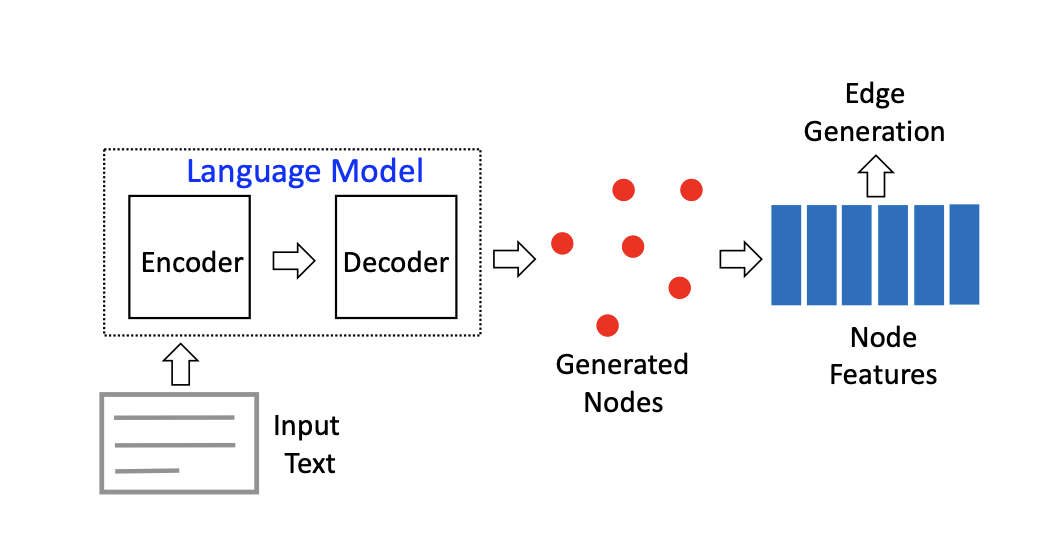
\includegraphics[width=0.8\textwidth]{img/Idea.png}
%   \caption{High level overview of constructing Knowledge Graphs from Language models}
%   \label{fig:kg_construction}
%   \end{figure}
  
\textbf{\cite{gao2023chatrec}} propose a novel paradigm called \textbf{Chat-Rec}, which augments large language models (LLMs) to build conversational recommender systems. This system converts user profiles and historical interactions into prompts, making the recommendation process more interactive and explainable. \textbf{Chat-Rec} is effective in learning user preferences and establishing connections between users and products through in-context learning. Moreover, it addresses challenges such as cold-start scenarios with new items and cross-domain recommendations, demonstrating improved performance in top-k recommendations and zero-shot rating prediction tasks.

Each of these papers contributes to the field of knowledge graph construction, embedding, and recommendation systems by introducing novel methods and techniques to enhance the quality and efficiency of knowledge representation and recommendation. By leveraging the power of large language models and graph neural networks, these models demonstrate the potential to improve the performance and interpretability of recommendation systems, paving the way for more effective and scalable knowledge-based recommendations.

\section{Exploratory Data Analysis}

\subsection{Exploratory Data Analysis}

This section aims to provide a comprehensive understanding of the dataset used for the research project. It contains information on the data source and files, as well as a description of the data's basic features. 

By performing exploratory data analysis (EDA), we aim to gain a deeper understanding of the data, including the relationship between variables and identifying trends. This analysis will inform the subsequent steps in the research and help address the research questions effectively.

\subsection{Data Source and Files}

The primary dataset in scope is \href{https://amazon-reviews-2023.github.io/index.html}{Amazon Reviews'23}. This is a large-scale Amazon Reviews dataset, collected in 2023 by McAuley Lab, and it includes rich features such as:
\begin {itemize}
\item User Reviews (ratings, text, helpfulness votes, etc.);
\item Item Metadata (descriptions, price, raw image, etc.);
\item Links (user-item / bought together graphs).
\end {itemize}

The datasets are open-sourced and compliant with the MRP requirements. 

The reviews span from May'96 to Sep'24 and cover a wide range of categories, including electronics, books, movies, and more. The dataset is designed to facilitate research in recommendation systems, natural language processing, and other related fields.


\subsection{Data Description}

For each category in the dataset, there are two main files: \textit{User Reviews} and \textit{Item Metadata}. The User Reviews file contains information about the reviews posted by users, including ratings, text, helpfulness votes, and more. The Item Metadata file contains information about the items being reviewed, such as descriptions, prices, images, and more.

\subsubsection{For User Reviews}
\begin{table}[H]
  \centering
  \begin{tabular}{|l|l|p{8cm}|}
  \hline
  \textbf{Field} & \textbf{Type} & \textbf{Explanation} \\ \hline
  rating & float & Rating of the product (from 1.0 to 5.0). \\ \hline
  title & str & Title of the user review. \\ \hline
  text & str & Text body of the user review. \\ \hline
  images & list & Images that users post after they have received the product. Each image has different sizes (small, medium, large), represented by the small\_image\_url, medium\_image\_url, and large\_image\_url respectively. \\ \hline
  asin & str & ID of the product. \\ \hline
  parent\_asin & str & Parent ID of the product. \\ \hline
  user\_id & str & ID of the reviewer. \\ \hline
  timestamp & int & Time of the review (unix time). \\ \hline
  verified\_purchase & bool & User purchase verification. \\ \hline
  helpful\_vote & int & Helpful votes of the review. \\ \hline
  \end{tabular}
  \caption{User Reviews Data Fields}
  \label{table:user_reviews}
  \end{table}
  
\subsubsection{For Item Metadata}

\begin{table}[H]
  \centering
  \begin{tabular}{|l|l|p{8cm}|}
  \hline
  \textbf{Field} & \textbf{Type} & \textbf{Explanation} \\ \hline
  main\_category & str & Main category (i.e., domain) of the product. \\ \hline
  title & str & Name of the product. \\ \hline
  average\_rating & float & Rating of the product shown on the product page. \\ \hline
  rating\_number & int & Number of ratings in the product. \\ \hline
  features & list & Bullet-point format features of the product. \\ \hline
  description & list & Description of the product. \\ \hline
  price & float & Price in US dollars (at time of crawling). \\ \hline
  images & list & Images of the product. Each image has different sizes (thumb, large, hi\_res). The ``variant'' field shows the position of image. \\ \hline
  videos & list & Videos of the product including title and url. \\ \hline
  store & str & Store name of the product. \\ \hline
  categories & list & Hierarchical categories of the product. \\ \hline
  details & dict & Product details, including materials, brand, sizes, etc. \\ \hline
  parent\_asin & str & Parent ID of the product. \\ \hline
  bought\_together & list & Recommended bundles from the websites. \\ \hline
  \end{tabular}
  \caption{Item Metadata Fields}
  \label{table:item_metadata}
  \end{table}

\subsection{Data Analysis}

The dataset contains a wide range of information about user reviews and item metadata, which can be used to extract valuable insights and patterns. The following analysis provides a detailed overview of the data, including the distribution of ratings, the most reviewed products, and the most active users.

We limit our analysis to the Books category for the purpose of this document, due to the large size of the dataset and the need to focus on a specific category for detailed analysis.

\subsubsection{Ratings Distribution}

The ratings distribution of the user reviews shown in fig \autoref{fig:ratings_distribution}  provides insights into the overall sentiment of the users towards the products. The distribution of ratings can help identify the most popular products and the products that need improvement. The following histogram shows the distribution of ratings in the dataset.

\begin{figure}[H]
\centering
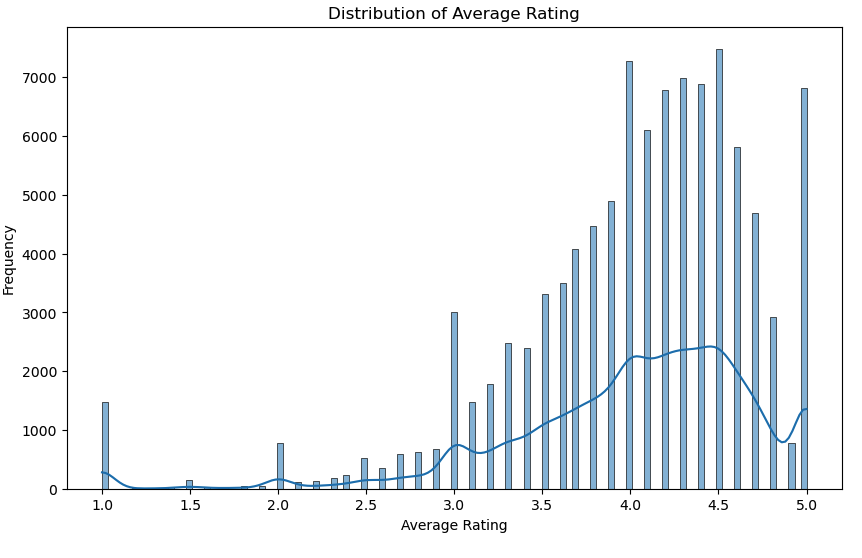
\includegraphics[width=0.8\textwidth]{img/avg_rating.png}
\caption{Ratings Distribution of User Reviews}
\label{fig:ratings_distribution}
\end{figure}

The ratings distribution shows that the majority of the reviews have high ratings, with a peak at 5.0. This indicates that users generally have positive sentiments towards the products they review. However, there are also reviews with lower ratings, indicating that some products may need improvement.

\subsubsection{Average Rating Over Time}

The trend of average product ratings from 1998 to 2022 is shown in \autoref{fig:avg_rating}. The graph reveals an initial decline in ratings until 2007, followed by a gradual increase peaking around 2015, and then a slight downward trend with fluctuations in recent years.
\begin{figure}[H]
\centering
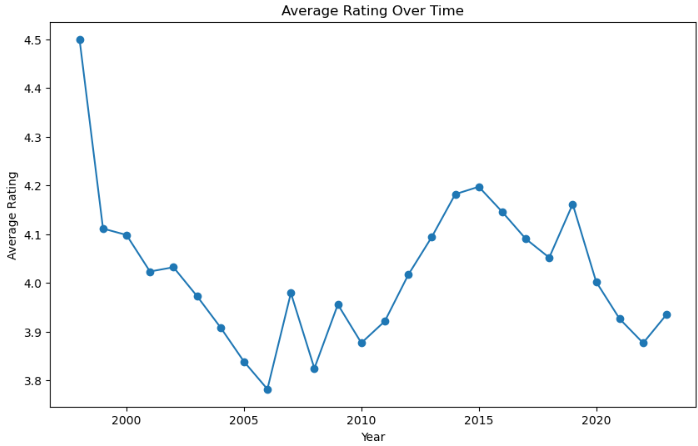
\includegraphics[width=0.8\textwidth]{img/avg_rating_over_time.png}
\caption{Average Rating Over Time}
\label{fig:avg_rating}
\end{figure}

\subsubsection{Number of Reviews Over Time}

\autoref{fig:review_count} displays the volume of reviews from 1999 to 2022. The graph shows exponential growth in review numbers, particularly steep from 2009 onwards, with significant fluctuations after 2014 and a sharp decline towards the end of the period.
\begin{figure}[H]
\centering
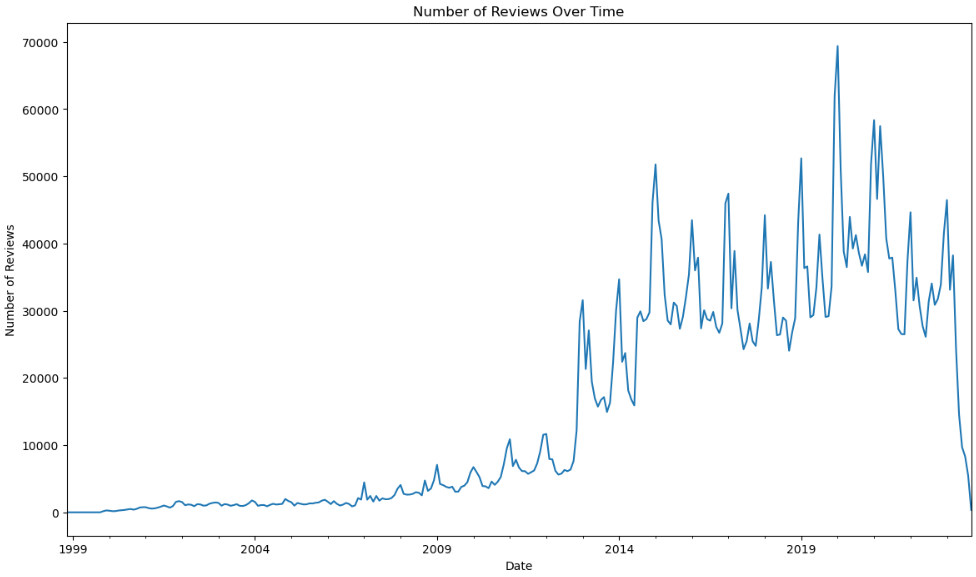
\includegraphics[width=0.8\textwidth]{img/no_reviews_over_time.png}
\caption{Number of Reviews Over Time}
\label{fig:review_count}
\end{figure}

\subsubsection{Word Cloud of Review Titles}

The word cloud in \autoref{fig:word_cloud} visualizes the most common words in review titles. It highlights the prevalence of star ratings, positive adjectives, and product-related terms, indicating customers' focus on ratings, overall satisfaction, and product functionality in their review titles.
\begin{figure}[H]
\centering
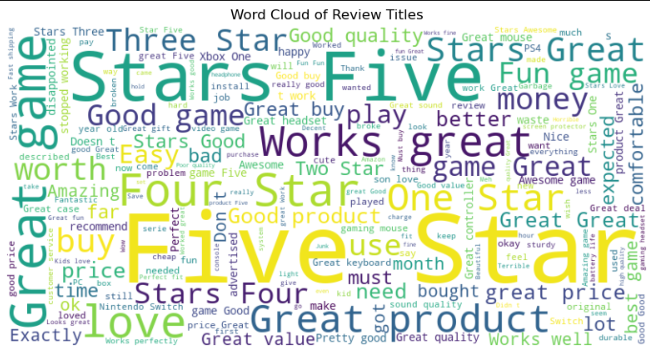
\includegraphics[width=0.8\textwidth]{img/wordcloud.png}
\caption{Word Cloud of Review Titles}
\label{fig:word_cloud}
\end{figure}

\section{Methodology}
Our approach consists of several interconnected stages, each contributing to the overall goal of creating an LLM-enhanced knowledge graph-based recommendation system. 

\subsection{Data Acquisition and Preprocessing} 
We will prepare the Amazon Reviews 2023 dataset first.
\begin{enumerate}
    \item \textbf{Dataset Acquisition:} 
    \begin{itemize}
        \item Obtain the Amazon Reviews 2023 dataset from the Hugging Face Hub.
        \item The dataset includes product reviews, metadata, and user information across multiple categories.
        \item We will focus on a specific category (e.g., Books) for detailed analysis and model development.
    \end{itemize}
    
    \item \textbf{Data Cleaning and Normalization:}
    \begin{itemize}
        \item Remove HTML tags, special characters, and irrelevant symbols from review texts and product descriptions.
        \item Normalize text data: convert to lowercase, remove extra whitespaces, and handle Unicode characters.
        \item Handle missing values through imputation or removal based on the nature of the missing data.
        \item Load the dataset into a database.
  
    \end{itemize}
    
    \item \textbf{Recommendation Preprocessing:}
        \begin{itemize}
            \item \textbf{K-Core Filtering}: Select a subset of users and items with a minimum number of interactions to reduce sparsity. 
            \begin{itemize}
                \item Due to the large size of the dataset, we will focus on a subset of users and items using k-core filtering e.g 15-core.
                \item Pros of high k-Core: Higher quality reviews, Reduced noise, Balanced distribution and Computational efficiency.
                \item Cons of high k-Core: Limited diversity, Misalignment with original data distribution, Loss of context, Generalizability and Limited data size for scaling up.
            \end{itemize}
        \end{itemize}
        \begin{itemize}
        \item \textbf{Leave-Last-Out Splitting:} A data-splitting strategy to pick up the lastest two item interactions for evaluation. This strategy is widely used in many recommendation papers.
    
        \begin{itemize}
            \item Training part: the first N-2 items;
            \item Validation part: the (N-1)-th item;
            \item Testing part: the N-th item.
        \end{itemize}
        \end{itemize}
        


    % \item \textbf{Text Preprocessing:}
    % \begin{itemize}
    %     \item Tokenization: Split text into individual words or subwords.
    %     \item Stop word removal: Eliminate common words that don't carry significant meaning.
    %     \item Lemmatization: Reduce words to their base or dictionary form.
    % \end{itemize}
    
\end{enumerate}

\subsection{Baseline Knowledge Graph Construction}
The baseline knowledge graph construction will involve creating a simple graph structure based on the existing metadata and relationships in the Amazon Reviews dataset.
\begin{enumerate}
    \item \textbf{Entity Extraction:}
    \begin{itemize}
        \item Identify key entities: product, category, features (e.g. price, rating, etc.). 
    \end{itemize}
    
    \item \textbf{Graph Structure Design:}
    \begin{itemize}
        \item Define node types e.g. Product, Category, Brand, Feature.
        \item Define edge types e.g. BelongsTo, HasFeature, CategorizedUnder.
    \end{itemize}
    
    \item \textbf{Graph Database Implementation:}
    \begin{itemize}
        \item Choose a scalable graph database (e.g., Neo4j).
        \item Develop efficient data ingestion pipelines to populate the graph database.
    \end{itemize}
\end{enumerate}

\subsection{Knowledge Graph Augmentation using LLM}
We will then use the LLM capabilities to enrich the knowledge graph with additional entities, attributes, and relationships extracted from the review texts and product descriptions.
\begin{enumerate}
    \item \textbf{Entity Enrichment:}
    \begin{itemize}
        \item Use the LLM to identify additional entities and attributes from review texts and product descriptions.
        \item Implement a confidence scoring mechanism for LLM-generated entities and attributes.
    \end{itemize}
    
    \item \textbf{Relationship Inference:}
    \begin{itemize}
        \item Leverage the LLM to infer complex relationships between entities (e.g., product similarities, complementary products).
        \item Develop a validation mechanism to verify LLM-inferred relationships against existing knowledge graph structures.
    \end{itemize}
    
    \item \textbf{Semantic Embedding Integration:}
    \begin{itemize}
        \item Generate semantic embeddings for products and reviews using the fine-tuned LLM.
        \item Integrate these embeddings as node properties in the knowledge graph to enhance similarity computations.
    \end{itemize}

\end{enumerate}


\subsection{LLM Integration and Fine-tuning}
\begin{enumerate}
    \item \textbf{LLM Selection:}
    \begin{itemize}
        \item Evaluate state-of-the-art LLMs (e.g., GPT-3, BERT, T5) based on performance metrics and resource requirements.
    \end{itemize}
    
    \item \textbf{Domain Adaptation:}
    \begin{itemize}
        \item Fine-tune the selected LLM on a subset of the Amazon Reviews data if necessary.
    \end{itemize}
    
    \item \textbf{Task-Specific Fine-tuning:}
    \begin{itemize}
        \item Develop specialized models for key tasks: entity recognition, relationship extraction, sentiment analysis.
        \item Implement few-shot learning techniques to adapt the LLM for specific product categories.
    \end{itemize}
    
    \item \textbf{Prompt Engineering:}
    \begin{itemize}
        \item Design effective prompts for various tasks: entity extraction, relationship inference, attribute generation.
        \item Develop a prompt library for consistent interactions with the LLM across different components of the system.
    \end{itemize}
\end{enumerate}


\subsection{Graph Embedding and Recommendation Algorithm Development}
\begin{enumerate}
    \item \textbf{Graph Embedding:}
    \begin{itemize}
        \item Implement a graph embedding model (e.g., TransE, ComplEx) to learn structured representations of entities and relationships in the knowledge graph.
    \end{itemize}
    
    \item \textbf{Recommendation Algorithm Design:}
    \begin{itemize}
        \item Implement a graph-based recommendation algorithm that leverages the graph embeddings as a side information source.
        \item Combine traditional collaborative filtering with graph-based approach.
    \end{itemize}
    
\end{enumerate}

\subsection{Evaluation and Optimization}
\begin{enumerate}
    \item \textbf{Offline Evaluation:}
    \begin{itemize}
        \item Split  data into train, validation, and test sets.
        \item Implement standard evaluation metrics: NDCG, Precision@k, Recall@k.
        \item Compare the peformance of the recommendation system system against baselines (e.g., standard collaborative filtering, non-LLM graph-based approaches).
        \item Develop graph-specific metrics to evaluate the quality of the knowledge graph and its impact on recommendations.
    \end{itemize}
    
\end{enumerate}

\section{Experiments}

To evaluate the effectiveness of our LLM-enhanced knowledge graph-based recommendation system, we will conduct a series of experiments. These experiments are designed to assess the impact of various components of our system and compare its performance against baseline methods.

\subsection{Experimental Setup}

\subsubsection{Dataset}
We will use the Amazon Reviews 2023 dataset, focusing on the Books category. The dataset will be split into 70\% training, 15\% validation, and 15\% test sets, ensuring temporal consistency to simulate real-world scenarios.

\subsubsection{Baselines}
We will compare our proposed method against the following baselines:
\begin{itemize}
    \item Collaborative Filtering (CF): A standard matrix factorization-based CF approach.
    \item Content-Based Filtering (CBF): Using TF-IDF vectors from product descriptions.
    \item Simple Graph-Based Recommendation (SGR): A graph-based method without LLM enhancements.
\end{itemize}

\subsubsection{Evaluation Metrics}
We will use the following metrics for evaluation:
\begin{itemize}
    \item Normalized Discounted Cumulative Gain (NDCG@k) for k = 5, 10
    \item Precision@k and Recall@k for k = 5, 10
\end{itemize}

\subsection{Experiment 1: Impact of LLM-based Knowledge Graph Augmentation}

This experiment will aim to evaluate the effectiveness of using LLM for knowledge graph augmentation.

\subsubsection{Method}
We will compare three versions of our system:
\begin{enumerate}
    \item Baseline KG: Using only metadata for graph construction.
    \item LLM-Entity KG: Baseline KG augmented with LLM-extracted entities.
    \item Full LLM-KG: LLM-Entity KG further augmented with LLM-inferred relationships.
\end{enumerate}

\subsubsection{Expected Outcome}
We will present a table or graph showing the performance metrics for each version. The discussion will focus on the impact of LLM-based augmentation on recommendation quality.

\begin{table}[h]
    \centering
    \begin{tabular}{|l|r|}
        \hline
        \textbf{Metric}             & \textbf{Value} \\ \hline
        Total Nodes                 & 157828         \\
        Total Relationships         & 331029         \\
        Graph Density               & 2.7e-05        \\
        % Avg Clustering Coefficient  & 0              \\
        Avg Node Properties         & 2.18           \\
        % Avg Relationship Properties & 0.0            \\
        % Isolated Nodes              & 0              \\
        Min Degree                  & 1              \\
        Max Degree                  & 37911          \\
        Avg Degree                  & 4.19           \\
        Median Degree               & 1.0            \\
        \hline
        Nodes by Label              &                \\
        \quad VideoGame             & 41659          \\
        \quad Store                 & 9545           \\
        \quad Category              & 165            \\
        \quad Feature               & 106459         \\
        \hline
        Relationships by Type       &                \\
        \quad BELONGS\_TO            & 41837          \\
        \quad CATEGORIZED\_UNDER     & 162432         \\
        \quad HAS\_FEATURE           & 126760         \\
        \hline
    \end{tabular}
    \caption{Neo4j Graph Statistics}
    \label{tab:neo4j-stats}
\end{table}

% \subsection{Experiment 2: Comparison of Graph Embedding Techniques}

% This experiment will compare different graph embedding techniques to determine the most effective approach for our recommendation system.

% \subsubsection{Method}
% We will test the following graph embedding methods:
% \begin{itemize}
%     \item TransE
%     \item ComplEx
%     \item RotatE
%     \item DistMult
% \end{itemize}

% \subsubsection{Expected Outcome}
% We will include a table or graph comparing the performance of different embedding techniques. The discussion will cover the strengths and weaknesses of each embedding technique in the context of our recommendation task.

\subsection{Experiment 2: LLM Fine-tuning Strategies}

This experiment will explore different fine-tuning strategies for the LLM to optimize its performance in knowledge graph augmentation and recommendation tasks.

\subsubsection{Method}
We will compare the following fine-tuning approaches:
\begin{itemize}
    \item No fine-tuning (off-the-shelf LLM)
    \item Full fine-tuning on Amazon Reviews data
    \item Task-specific fine-tuning (entity extraction, relationship inference)
    \item Few-shot learning with prompt engineering
\end{itemize}

\subsubsection{Expected Outcome}
We will present a table or graph showing the performance of each fine-tuning strategy. The discussion will focus on the trade-offs between different fine-tuning strategies in terms of performance and computational requirements.

\subsection{Experiment 3: Scalability and Efficiency Analysis}

This experiment will assess the scalability and computational efficiency of our proposed system compared to baseline methods.

\subsubsection{Method}
We will measure the following metrics:
\begin{itemize}
    \item Training time
    \item Inference time for recommendations
    \item Memory usage
    \item Scaling behavior with increasing dataset size
\end{itemize}

\subsubsection{Expected Outcome}
We will include graphs or tables showing scalability and efficiency metrics. The discussion will cover the practical implications of the scalability and efficiency results.

% \subsection{Experiment 5: Cold Start Problem}

% This experiment will evaluate how well our system handles the cold start problem compared to baseline methods.

% \subsubsection{Method}
% We will simulate cold start scenarios by:
% \begin{itemize}
%     \item Removing a subset of users/items from the training data
%     \item Evaluating recommendations for these "new" users/items
% \end{itemize}

% \subsubsection{Expected Outcome}
% We will present a table or graph comparing cold start performance. The discussion will focus on how the LLM-enhanced knowledge graph approach addresses the cold start problem.

% \subsection{Conclusion}
% Upon completion of these experiments, we will summarize the key findings and their implications for the proposed recommendation system. This comprehensive evaluation will provide insights into the effectiveness of our LLM-enhanced knowledge graph-based approach and its potential advantages over existing methods.
% \section{Conclusion}


\section{Conclusion}

This document provides a comprehensive overview of the methodology conducted for the second deliverable of the Major Research Project.

This methodology outlines a comprehensive approach to creating an LLM-enhanced knowledge graph-based recommendation system using the Amazon Reviews 2023 dataset. 

By leveraging the semantic understanding capabilities of LLMs and the structured representation of knowledge graphs, we aim to develop a more intelligent and context-aware recommendation system.


\section{Future Work}

The next steps in the research project will focus on the implementation and evaluation of the proposed methodology. 

Future work will focus on implementing this methodology and conducting extensive experiments to validate its effectiveness in real-world e-commerce scenarios.

\printbibliography
\clearpage

\appendix

\end{document}
